\section{Finite Markov Decision Processes}

MDP Formulation: $ s_t, a_t \to r_{t+1}, s_{t+1} $

\begin{figure}[h]
    \centering
    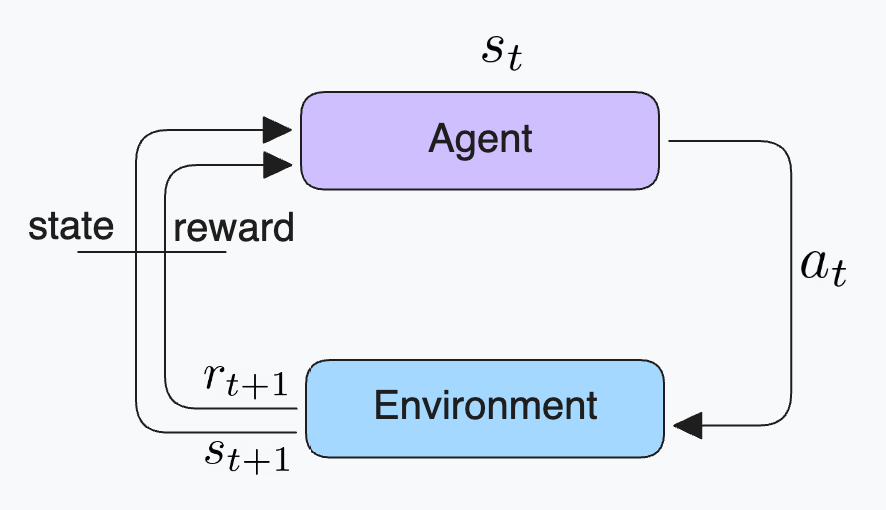
\includegraphics[width=0.9\textwidth]{img/mdp_setting.png}
    \caption{MDP Formulation.}
    \label{fig:mdp}
\end{figure}

$p(s', r | s, a)$ is the probability of transitioning to state $s'$ and receiving reward $r$
given that we are in state $s$ and take action $a$. The current state $s_t$ includes all the
information about the past. (i.e., the Markov property)

The state transition probability is given by:
 \begin{equation}
    \begin{split}
        p(s'|s, a) = \sum_{r} p(s', r | s, a) \\
        \label{eq:mdp-transition-probability}
    \end{split}
 \end{equation}

The reward function is given by:
 \begin{equation}
    \begin{split}
        r(s, a) = \mathbb{E}[R_{t+1} | S_t = s, A_t = a] \\
        = \sum_{r} r \sum_{s'} p(s',r|s, a) \\
        \label{eq:mdp-reward-function}
    \end{split}
 \end{equation}

The MDP is defined by the tuple $(S, A, p, r, \gamma)$, where $S$ is the state space, $A$ is the
action space, $p$ is the state transition probability, $r$ is the reward function, and $\gamma$
is the discount factor.

Goal: Maximize expected (discounted) return over time, with discount factor $\gamma \in [0, 1]$.


\begin{equation} 
    \begin{split}
        G_t = R_{t+1} + \gamma R_{t+2} + \gamma^2 R_{t+3} + \cdots \\
        \label{eq:mdp-return}
        G_t = R_{t+1} + \gamma G_{t+1} \quad \textit{(recursive definition)} \\ 
        = \sum_{k=0}^{\infty} \gamma^k R_{t+k+1} \quad \textit{(infinite sum)} \\
    \end{split}
 \end{equation}

\subsection{Policy and Value Functions}
A policy $\pi(a|s)$ is a mapping from states to actions indicating the probability of taking action $a$ in state $s$.

The \textbf{state-value function} $v_\pi(s)$ is the expected return starting from state $s$ and following policy $\pi$.

\begin{equation}
    \begin{split}
        v_\pi(s) = \mathbb{E}[G_t | S_t = s] \quad \text{for all } s \in S \\
        \label{eq:mdp-value-function}
    \end{split}
 \end{equation}

The \textbf{action-value function} $q_\pi(s, a)$ is the expected return starting from state $s$, taking action $a$, and following policy $\pi$.

\begin{figure}[h]
    \centering
    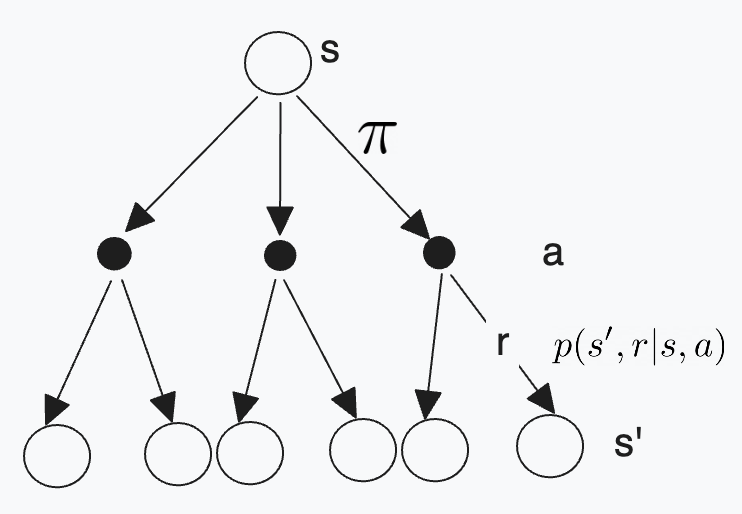
\includegraphics[width=0.9\textwidth]{img/backup_diagram1.png}
    \caption{General setting of MDP.}
    \label{fig:mdp-back-up-diagram}
 \end{figure}

\begin{equation}
    \begin{split}
        q_\pi(s, a) = \mathbb{E}[G_t | S_t = s, A_t = a] \\
        \label{eq:mdp-action-value-function}
    \end{split}
 \end{equation}

 Expected reward at time $t$ is given by:
 \begin{equation}
    \begin{split}
        \mathbb{E}[R_{t+1} | S_t = s, A_t = a] = \sum_{r} r \sum_{s'} p(s',r|s, a) \\
        = \sum_{a} \pi(a|s) \sum_{s',r} r . p(s',r|s, a) \\
        \label{eq:mdp-expected-reward}
    \end{split}
 \end{equation}

 \begin{equation}
    \begin{split}
        v_\pi(s) = \mathbb{E}[G_t | S_t = s]  \\
         = \sum_{G_t} G_t . p(G_t | S_t = s) \\
         = \sum_{G_t} G_t . p(R_t | S_t = s) \\
         = \sum_{G_t} G_t . \sum_{a} \pi(a|s) \sum_{s'} p(s'|s, a) \\
         = \sum_{G_t} G_t . \sum_{a} \pi(a|s) \sum_{s',r} p(s',r|s, a) \\
         v_\pi(s)  = \sum_{a} \pi(a|s) q_\pi(s, a) \\
        \label{eq:mdp-bellman-equation}
    \end{split}
 \end{equation}

 \begin{figure}[h]
    \centering
    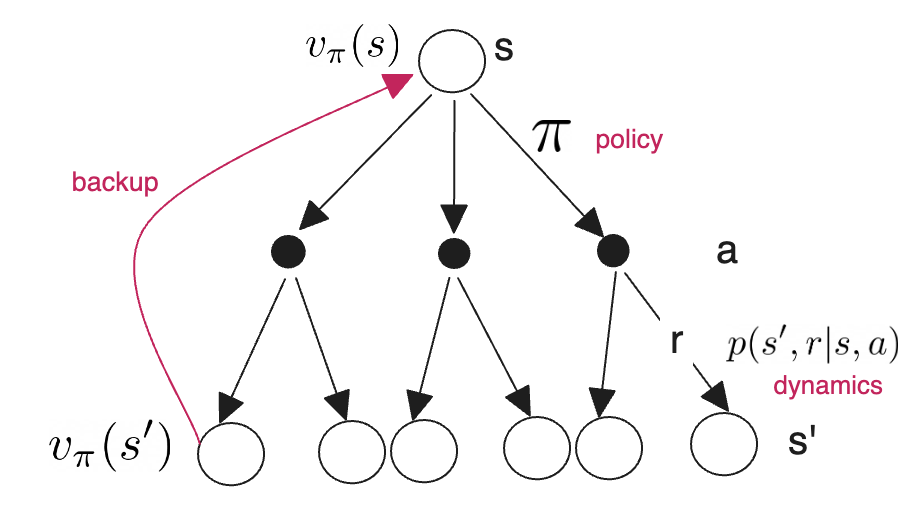
\includegraphics[width=0.9\textwidth]{img/backup_diagram2.png}
    \caption{Back-up diagram for the value function.}
    \label{fig:mdp-back-up-diagram}
 \end{figure}


 Furthermore, the value function can be decomposed into the immediate reward plus the discounted value of the next state:
 \begin{equation}
    \begin{split}
        v_\pi(s) = \mathbb{E}[R_{t+1} + \gamma G_{t+1} | S_t = s] \\
        v_\pi(s) = \sum_{a} \pi(a|s) \sum_{s',r} p(s',r|s, a) [r + \gamma v_\pi(s')] \\
        \label{eq:mdp-bellman-equation-2}
    \end{split}
 \end{equation}

 This is the \textbf{Bellman equation} for the value function $v_\pi$, averaging over all possible next actions, weighted
 by the probability of occuring.

The \textbf{Bellman equation} for the action-value function $q_\pi(s, a)$ is given by:

  \begin{equation}
    \begin{split}
       q_\pi(s, a) = \mathbb{E}[R_{t+1} + \gamma G_{t+1} | S_t = s, A_t = a] \\
       q_\pi(s, a) = \sum_{s',r} p(s',r|s, a) [r + \gamma v_\pi(s')] \\
       \label{eq:mdp-bellman-equation-3}
    \end{split}
 \end{equation}

 Derivation below:
 \begin{equation}
    \begin{split}
        q_\pi(s, a) = \mathbb{E}[R_{t+1} + \gamma G_{t+1} | S_t = s, A_t = a] \\
        = \mathbb{E}[R_{t+1} | S_t = s, A_t = a]  + \gamma \mathbb{E}[G_{t+1} | S_t = s, A_t = a] \\
        = \sum_{r,s'} r . p(s',r|s, a) + \gamma \sum_{s'} v_\pi(s') p(s'|s, a) \\
        = \sum_{s',r} p(s',r|s, a) [r + \gamma v_\pi(s')] \\
        \label{eq:mdp-bellman-equation-4}
    \end{split}
 \end{equation}

 In summary,

 \begin{equation}
    \begin{split}
        v_\pi(s) = \sum_{a} \pi(a|s) q_\pi(s, a) \\
        v_\pi(s) = \sum_{a} \pi(a|s) \sum_{s',r} p(s',r|s, a) [r + \gamma v_\pi(s')] \\
        q_\pi(s, a) = \sum_{s',r} p(s',r|s, a) [r + \gamma v_\pi(s')] \\
        q_\pi(s, a) = \sum_{s',r} p(s',r|s, a) [r + \gamma \sum_{a'} \pi(a'|s') q_\pi(s', a')] \\
        \label{eq:mdp-bellman-equation-5}
    \end{split}
 \end{equation}
